\documentclass{article}
\usepackage[utf8]{inputenc}
\usepackage{polski}
\usepackage{geometry}
\usepackage{pdfpages}
\usepackage{pdfpages}
\usepackage{listings}
\usepackage{listingsutf8}
\usepackage{multirow}
\usepackage{siunitx}
\usepackage{multirow}
\usepackage{booktabs}
\usepackage{tabularx}
\usepackage{placeins}
\usepackage{pdflscape}
\usepackage{graphicx}
\usepackage{subfig}
\usepackage{hyperref}
\usepackage{amsmath}
\usepackage{colortbl}

\geometry{
a4paper,
total={170mm,257mm},
left=20mm,
top=20mm
}
\newcolumntype{Y}{>{\centering\arraybackslash}X}
% \renewcommand\thesection{}
\lstset{%
literate=%
 {ą}{{\k{a}}}1
 {ę}{{\k{e}}}1
 {Ą}{{\k{A}}}1
 {Ę}{{\k{E}}}1
 {ś}{{\'{s}}}1
 {Ś}{{\'{S}}}1
 {ź}{{\'{z}}}1
 {Ź}{{\'{Z}}}1
 {ń}{{\'{n}}}1
 {Ń}{{\'{N}}}1
 {ć}{{\'{c}}}1
 {Ć}{{\'{C}}}1
 {ó}{{\'{o}}}1
 {Ó}{{\'{O}}}1
 {ż}{{\.{z}}}1
 {Ż}{{\.{Z}}}1
 {ł}{{\l{}}}1
 {Ł}{{\l{}}}1
}

\title{Systemy Rozproszone\\ 
Laboratorium II - RabbitMQ}
\author{Maciej Trątnowiecki}
\date{AGH, Semestr Letni, 2021}

\begin{document}
    \maketitle
    \lstset{ 
      backgroundcolor=\color{white},   % choose the background color; you must add \usepackage{color} or \usepackage{xcolor}; should come as last argument
      basicstyle=\footnotesize,        % the size of the fonts that are used for the code
      breakatwhitespace=false,         % sets if automatic breaks should only happen at whitespace
      breaklines=true,                 % sets automatic line breaking
      captionpos=b,                    % sets the caption-position to bottom
      commentstyle=\color{mygreen},    % comment style
      deletekeywords={...},            % if you want to delete keywords from the given language
      escapeinside={\%*}{*)},          % if you want to add LaTeX within your code
      %extendedchars=true,              % lets you use non-ASCII characters; for 8-bits encodings only, does not work with UTF-8
      firstnumber=1000,                % start line enumeration with line 1000
      frame=single,	                   % adds a frame around the code
      keepspaces=true,                 % keeps spaces in text, useful for keeping indentation of code (possibly needs columns=flexible)
      keywordstyle=\color{blue},       % keyword style
      language=Octave,                 % the language of the code
      morekeywords={*,...},            % if you want to add more keywords to the set
      numbers=left,                    % where to put the line-numbers; possible values are (none, left, right)
      numbersep=5pt,                   % how far the line-numbers are from the code
      numberstyle=\tiny\color{mygray}, % the style that is used for the line-numbers
      rulecolor=\color{black},         % if not set, the frame-color may be changed on line-breaks within not-black text (e.g. comments (green here))
      showspaces=false,                % show spaces everywhere adding particular underscores; it overrides 'showstringspaces'
      showstringspaces=false,          % underline spaces within strings only
      showtabs=false,                  % show tabs within strings adding particular underscores
      stepnumber=2,                    % the step between two line-numbers. If it's 1, each line will be numbered
      stringstyle=\color{mymauve},     % string literal style
      tabsize=2,	                   % sets default tabsize to 2 spaces
      title=\lstname                   % show the filename of files included with \lstinputlisting; also try caption instead of title
    }
    
    \section{Obserwacja mechanizmu niezawodności kolejki}
        W celu przeprowadzenia obserwacji przetestowałem działanie systemu dla trzech sposobów potwierdzeń otrzymania wiadomośći. 
        \begin{itemize}
            \item Potwierdzenia wysyłane przez RabbitMQ API po otrzymaniu wiadomości
            \item Potwierdzenia wysyłane ręcznie po przetworzeniu wiadomości 
            \item Brak potwierdzeń
        \end{itemize}
        Najwyższą niezawodność zapewniają potwierdzenia przesyłane po zakończeniu przetwarzania wiadomości. W ten sposób otrzymujemy system odporny na przerwanie przetwarzania otrzymanej już wiadomości w przypadku wystąpienia błędu - w tej sytuacji proces konsumenta będzie ponownie otrzymywał nieprzetworzoną wiadomość aż do otrzymania przez serwer kolejki potwierdzenia informującego o poprawnym zakończeniu przetwarzania. \\
        W przypadku automatycznego wysyłania potwierdzenia po odbiorze wiadomości serwer nie gwarantuje jej przetworzenia. To jest, w przypadku przerwania przetwarzania w wyniku błędu w procesie konsumenta, system nigdy nie spróbuje ponownie przetworzyć otrzymanej wiadomości. \\
        Jeśli nie zapewnimy przesyłania potwierdzeń w żaden sposób, serwer będzie ponownie wysyłał te same wiadomości do procesu konsumenta, nawet jeśli zostały już przetworzone kilkukrotnie. Każda nowa wiadomość będzie dodawana na koniec kolejki nieprzerwania przesyłanych wiadomości. 
        
    \section{Obserwacja mechanizmu równoważenia obciążenia}
        W ramach obserwacji wysłałem kolejno 10 wiadomości, obsługiwanych przez dwóch klientów. Poniżej zamieszczam wyjście klientów z wyłączon i z włączoną funkcją QOS.
        \lstinputlisting[language=bash]{no_qos.txt}
        \lstinputlisting[language=bash]{qos.txt}
        Możemy zauważyć, że w wersji bez QOS wiadomości których przetwarzanie zajmuje dużo czasu obsługiwane są zawsze przez tego samego klienta, pomimo że pierwszy klient kończy przetwarzanie dużo szybciej. Dzieje się tak dlatego, RabbitMQ rozdziela wiadomości w momencie w którym dochodzą do kolejki równomiernie pomiędzy klientów, nie biorąc pod uwagę potwierdzeń o ich przetworzeniu. W naszym przypadku pierwszy klient otrzymuje zawsze parzyste, a drugi nieparzyste z wiadomości. \\
        Po włączeniu obsługi funkcji QOS z argumentem $1$ w klientach kolejki, RabbitMQ nie przydzieli żadnemu z klientów więcej niż jednej wiadomości na raz. To znaczy, że dopóki klient nie zakończy przetwarzania wiadomości, nie otrzyma kolejnej. Dzięki temu, czas w jakim klient przetworzył wiadomość (a konkretniej w jakim wyśle potwierdzenie) wpływa pośrednio na to, kiedy otrzyma następną wiadomość. W wyjściach klientów obserwujemy bardziej równomierne rozłożenie wiadomości.
        
    \section{Routing Direct oraz Topic}
        Wyobraźmy sobie system rozproszony, który przetwarza pewne dane. Może on przesyłać przetwarzane dane pomiędzy węzłami z wykorzystaniem serwera RabbitMQ. Niech "producent" umieszcza odczytane z dysku dane w formie wiadomości w systemie, oznaczając typ przesyłanych danych kluczem w umieszczanej wiadomości. 
        Niech klucz zawiera informację o formacie przesyłanego pliku, tj. \texttt{[csv|json|png|mov]}. 
        Załóżmy, że dla każdego z czterech wykorzystywanych w tym eksperymencie formatów plików musimy zaimplementować odpowiedni wyspecjalizowany węzeł zdolny do przetworzenia takich danych w pewien sobie tylko znany sposób.\\
        Do implementacji takiego systemu możemy wykorzystać exchanger typu direct. Dla każdego z czterech możliwych kluczy definiujemy wprost węzeł docelowy wiadomości. 
        \begin{center}
            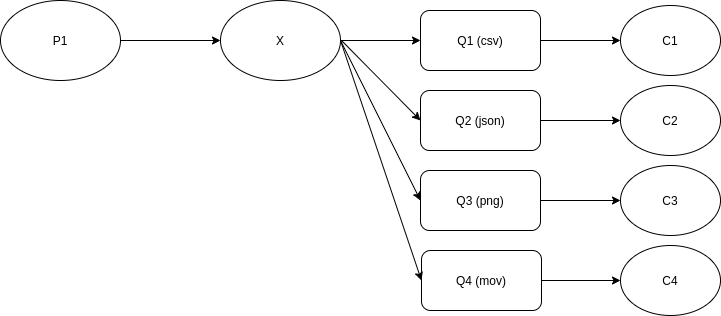
\includegraphics[width=13cm]{lab2/report/ex3_1.png}
        \end{center}\\
        Teraz wyobraźmy sobie, że oprócz przetworzenia każdej wiadomości na jednym z czterech zdefiniowanych powyżej węzłów, chcemy wykonać pewne dodatkowe zadania. Przykładowo, chcemy każdą wiadomość tekstową zapisać w pewnym logu, a każdą wiadomość z plikiem multimedialnym odesłać do odpowiedniego działu firmy w celu weryfikacji pod kątem treści nieodpowiednich.\\
        % \newpage
        Zmodyfikujmy format klucza przesyłanych wiadomości. Niech klucz będzie zgodny z formatem:\\ \texttt{[text|media].[csv|json|png|mov]}. Pierwszy człon klucza określa czy dane są typu tekstowego, drugi człon koduje informacje o formacie przesyłanych danych.\\
        W dodatu pliki json o rozmiarze zbyt dużym dla naszego mało wydajnego systemu logów chcemy móc oznaczyć kluczem media.json. Tak zaadresowana wiadomość nie powinna trafić do węzła obsługi logów.
        Do wykonania tak zaprojektowanego systemu wykorzystać możemy exchanger typu topic, np. w sposób zaprezentowany na poniższym diagramie. 
        \begin{center}
            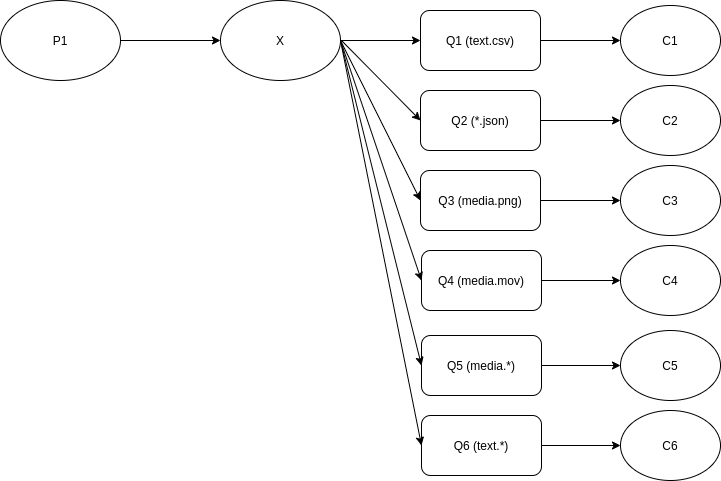
\includegraphics[width=13cm]{lab2/report/ex3_2.png}
        \end{center}\\
        Dla pierwszego przykładu konfiguracja systemu może wyglądać następująco. 
        \begin{enumerate}
            \item Klucze przy wiązaniu kolejek: \begin{itemize}
                \item Q1 - csv
                \item Q2 - json
                \item Q3 - png
                \item Q4 - mov
                \end{itemize}
            \item Klucze w przesyłanych wiadomościach: kluczem każdej z wiadomości jest jedno z czterech słów - csv, json, png, mov
            \item Odbiorcy przykładowych wiadomości: każdy z odbiorców otrzymuje wiadomość o kluczach takich samych jak klucz przypisany do kolejki podczas wiązania
        \end{enumerate}
        Dla drugiego przykładu konfiguracja systemu może wyglądać następująco. 
        \begin{enumerate}
            \item Klucze przy wiązaniu kolejek: \begin{itemize}
                \item Q1 - text.csv
                \item Q2 - *.json
                \item Q3 - media.png
                \item Q4 - media.mov
                \item Q5 - media.*
                \item Q6 - text.*
                \end{itemize}
            \item Klucze w przesyłanych wiadomościach:
                Wiadomość może zawierać jeden z następujących kluczy:
                \begin{itemize}
                    \item text.csv
                    \item text.json
                    \item media.json
                    \item media.png
                    \item media.mov
                \end{itemize}
            \item Odbiorcy przykładowych wiadomości: 
                \begin{itemize}
                    \item text.csv - C1 oraz C6
                    \item text.json - C2 oraz C6
                    \item media.json - C2
                    \item media.png - C3 oraz C5
                    \item media.mov - C4 oraz C5
                \end{itemize}
        \end{enumerate}
\end{document}
